% ihope_pipeline.tex

% citation shortcuts
\def\12to18{Abbott:2009qj}
\def\sfive1yr{Collaboration:2009tt}
\def\sfivelvc{S5LowMassLV}


In this chapter we describe in detail the \ihope pipeline, which is the pipeline
used to carry out the \ac{CBC} search. This pipeline has been used to analyze
data taken from \ac{S5} \cite{\sfive1yr,\12to18}, \ac{S6}, \ac{VSR2}, and
\ac{VSR3} \cite{s6paper}.

\ihope can by modeled by a \ac{DAG}. A \ac{DAG} is a workflow in which the
output of one program, or {\it node}, is the input of another node or nodes,
such that the flow never loops back onto itself. It is represented by a diagram
in which the vertices are the programs and the edges show the interdependencies
\cite{condor}. \ihope is a \ac{DAG} of \ac{DAG}s: its nodes are workflows that
launch sub-workflows, which in-turn launch the programs that carry out the
analysis. These \ac{DAG}s are managed by the Condor High Throughput Computing
system, which distributes the jobs across the computer cluster and manages the
dependencies. Figure \ref{fig:ihopeOverview} shows an overview of the \ihope
workflow. Data from each \ac{IFO} is retrieved, analyzed in parallel workflows,
combined, and then output to a webpage. Each of these steps involves one or
more \ac{DAG}s.

In this chapter we go through each of these steps in detail. Section
\ref{sec:PipelineRequirements} reviews the requirements of a \ac{CBC} \ac{GW}
pipeline; section \ref{sec:ihopeRuntime} explains how the dag is set-up at
run-time; section \ref{sec:HIPEdetail} describes the HIPE pipeline in detail;
\ref{sec:TableStructure} describes the tables used to store data;
\ref{sec:PipedownDetail} describes Pipedown in detail and how the results are
presented. 

\begin{figure}[h]
\begin{center}
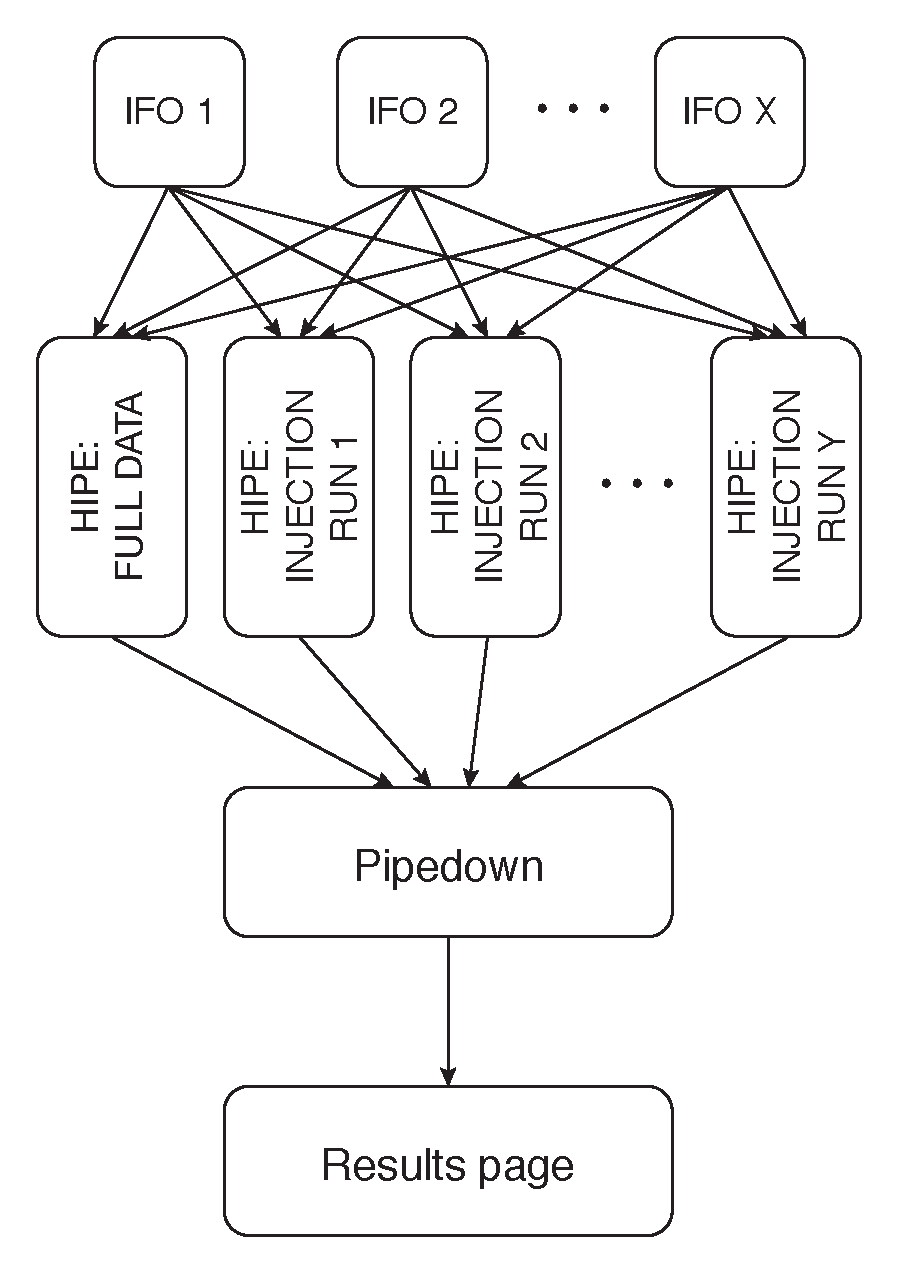
\includegraphics[width=2.5in]{figures/ihopeOverview.pdf}
\end{center}
\caption{
An overview of the \ihope pipeline. The HIPE and Pipedown nodes are themselves workflows, and are detailed in later sectionss.
}
\label{fig:ihopeOverview}
\end{figure}

\section{Pipeline Requirements}
\label{sec:PipelineRequirements}

Before delving into the details of \ihope, we briefly review the key
requirements of a pipeline used to search for \ac{GW}s. Our goal is to search
for \ac{GW}s from coalescing binaries in a range of masses. Hampering our
efforts is the fact that gravitational waves couple very weakly to matter; we
must be able to detect strains of $\sim10^{-21}$. Despite this, we
aim to detect at a \ac{SNR} of $8$ in each detector to ensure statistical
confidence in our search.

When averaged over time the detectors' have a colored-Gaussian noise
distrubtion; as shown in Chapter \ref{ch:pipeline_principles}, the best analysis tool to search for signals is therefore a
matched filter \cite{?}. Match filtering requires knowing the morphology of the
waveform. Fortunately, binaries with total masses (\mtotal) less than $25\Msun$
sweep through the \ac{LIGO} and Virgo bands during their {\it inspiral} phases.
This means that the waveform from these systems can be well modelled by the
post-Newtonian approximation. For higher-mass systems ($25 < \mtotal/\Msun <
100$), in which the merger and ringdown part of the waveform become important,
numerical relativity waveforms can be stiched to the \ac{pN} approximation;
phenomenological waveforms may also be used. Thus, to cover the desired range,
we can fill a bank of templates using the methods described in section \ref{sec:multiple_templates} of Chapter \ref{ch:pipeline_principles}.

Environmental and instrumental factors can cause non-Gaussian transient noise
(\emph{glitches}) in the data. To deal with this our pipeline must be able to
distinguish between triggers resulting from glitches and triggers resulting
from gravitational waves. Since the morhpology of the signals is known, the $\chi^2$ test discussed in \ref{ch:pipeline_principles} lends itself as a good method to do this. Checking for coincident triggers in multiple detectors will
also filter out spurious triggers since we do not expect environmental
correlations across great distances. After all filtering and tests have been
applied, the statistical significance of a set of triggers has to be evaluated
to determine the probability that a gravitational wave exists in the data. A
pipeline must therefore be able to compute a background with which to compare
triggers to. To avoid bias, this must be done in a {\it blind} fashion: the
method by which background is chosen and triggers ranked must be chosen without
knowledge of what is in the data, else the results will sway in the favor of the
analysts' bias. 

Finally, the pipeline must be able to evaluate its sensitivity and efficiency
to sources in the universe. Doing so allows tuning studies to be carried out
prior to doing the full analysis, and for the astrophysical rate of \ac{CBC}s
to be bounded after the analysis has completed. This can be done by performing
\emph{injections} of signals with known parameters into the detectors. Both \emph{hardware} and \emph{software} injections may be performed. Hardware injections
involve actuating the mirrors to physically simulate a passing gravitational
wave. This is the most robust test as it checks the ability of the detectors'
response loop to measure \ac{GW} strains and the ability of the pipeline to
detect them. The trouble with hardware injections is that real \ac{GW}s cannot
be detected while they are occurring, limiting the number that can be done.
Software injections involve adding a gravitational wave signal to the data
stream on disk just prior to analyzing it. While this method doesn't test the
hardware control systems, it has the advantage that it can be done many times
in parallel, without corrupting the original data. Thus, our pipeline must be
able to perform software injections, and have a method for associating triggers
with the injections that went into the data.

In summary, a pipeline used to search for gravitational waves from \ac{CBC}s must:
\begin{itemize}
\item{construct a bank of templates with which to filter;}
\item{identify \emph{triggers} by filtering templates through the detector data;}
\item{distinguish noise triggers from gravitational wave triggers;}
\item{quantify statistical significance of triggers and rank them in a blind manner;}
\item{evaluate the sensitivity and efficiency of the search to \ac{CBC}s in the universe.}
\end{itemize}
In the following sections we will see how \ihope meets these requirements.


\section{\ihope at Runtime}
\label{sec:ihopeRuntime}

The \ihope pipeline is created by running \texttt{lalapps\_ihope}. This sets up
the workflow by doing the following at run time:

\begin{itemize}
\item{set-up the directory structure to save all data to;}
\item{copy all needed programs from their installed location to a local directory;}
\item{retrieve analysis start and stop times;}
\item{download a {\it veto-definer file} and find the start and stop times of all veto segments;}
\item{run \texttt{lalapps\_inspiral\_hipe};}
\item{run \texttt{lalapps\_cbc\_pipedown};}
\item{create a cache file of the names and locations of all files that will be created;}
\item{write a DAX that can be used to start and run the worflow.}
\end{itemize}

These steps require the start and stop time (in GPS seconds) of the period to
be analyzed as well as a configuration file. The configuration file is a text
file containing all the information needed to setup and run the analysis. This
includes: the names and locations of all the executables that will be run;
variable arguments that these programs will need; the name and number of
interferometers to analyze; the version of data files to retrieve and what
channels to analyze; how many and what type of software injection runs to do;
any other information needed by the \ac{DAG}s to run. The configuration file
provides a convenient way to manipulate the pipeline. Changing tuning
parameters is largely accomplished by editing this file. Likewise, the
difference between running a {\it low-mass} search ($2 < \mtotal/\Msun < 25$)
and a {\it high-mass} search ($25 < \mtotal/\Msun < 100$) is determined
entirely by the configuration file.

A directory named by the gps start/stop times is created at runtime. All work
is done in this directory. In it, a \texttt{segments}, \texttt{executables},
\texttt{datafind}, \texttt{full\_data}, and \texttt{pipedown} directory are
created, along with a directory for each injection run that will be carried
out. With the exception of the \texttt{executables} and \texttt{segments}
directory, each of the sub directories store a sub-\ac{DAG} that will be run
during the analysis (and will be explained below). The master \ac{DAG} is saved
in the gps-times direcotory along with a master cache file of all the files
that will be created. All programs that will be run are copied to the
\texttt{executables} directory.

\subsection{Science and Veto Segments Retrieval}

The \ac{LIGO} and Virgo detectors can be in one of five different states at any
given time. We are only interested in analyzing times in which the detectors
are in {\it Science} mode. This means they are up, locked, and no other
experimental work is being done on them \cite{?}. The interferometers
can drop out of Science mode many times across an analysis period; thus \ihope
must retrieve the start and stop times of Science segments that occurred in the
desired analysis period. \ihope does this by running
\texttt{ligolw\_segment\_query} at run time. This program queries the {\it
segment database} --- a remote database that contains lists of segments
detailing the times that each of the detectors were in various states --- to
retrieve the list of Science times during the desired analysis period. These
results are saved to xml files in the \texttt{segments} directory. These files
do not contain strain data; they only list the times that data can be
retrieved. The results are later used to retrieve files containing strain data.

Various environmental and instrumental factors can cause periods of elevated
glitch rate during Science mode. If these periods are analyzed with periods of
relatively clean data, they will pollute the background estimation, thereby
decreasing statistical confidence in candidates. We therefore seek to remove
such periods from the analysis. This is accomplished using vetoes. Vetoes are
categorized according to how well we can couple them to known environmental
sources; they are applied cumulatively. Table \ref{tab:vetocats} lists the
various categories and their defining characteristics. For \ac{CBC} searches,
we do not analyze anything prior to category 1; i.e., all matched filtering is
done after category 1 vetoes are applied. Category 2 and 3 vetoes are applied
when second stage coincidence is carried out (see HIPE, below). We quote false
alarm rates and base upper limits on data in which category 1-3 vetoes have
been applied. We additionally check the data after category 1 and 2 vetoes have
been applied for any loud triggers that may have been removed by category 3
vetoes. We do not use category 4 for the anlaysis; however, we do use them in
follow-up studies of loud events to provide insight into the cause of the
events. Hardware injections are left in the data after category 1 and 2, and
are removed as a special veto prior to category 3 vetoes being applied.

\begin{table}
\center
\begin{tabular}{c | p{5cm} | p{8cm}}
Category    &    Description    &   Procedure    \\
\hline
    1       &    Data seriously compromised or missing.    &    Data never analyzed. \\
\hline
    2       &    Instrumental problems with known coupling to h(t).    &    Vetoed triggers discarded after second coincidence. Surviving triggers checked for candidates, but not used for upper limits. \\
\hline
    3       &    Instrumental problems likely, casting doubt on triggers found during these times.    &    Vetoed triggers discarded after second coincidence. False alarm rates of surviving triggers are used in publications; upper limits are calculated using these vetoes.  \\
\hline
    4       &    Positive, but weak, correlations with false alarms. Large dead times.    &     Not used in the analysis, but used as a guide in detailed followups of loud triggers. \\
\end{tabular}
\caption{The various veto categories used by the \ac{CBC} group. Vetoes are applied cumulatively; statistical significance of candidates and upper limits are calculated after category 1, 2, and 3 vetoes are applied.}
\label{tab:vetocats}
\end{table}

Vetoes are triggered by environmental and instrumental channels that flag
various segments of time for suspicious activity. Additional flags can be added
by hand; e.g., if a truck drives onto the site during Science mode, a person
in the control room may add a flag for that period of time. All of these flags
are stored in the segment database. What flags to use for vetoes, at what
category, and for how long, are stored in a \emph{veto-definer file}. This xml
file contains a \texttt{veto\_definer} table that lists each flag that should
be used, what category the flag should be used at, the dates the flag is valid, and any
padding (in seconds) to add to the flag should it go off. Entries are added to
this table by hand after extensive data-quality investigations and safety
checks. Vetoes are fine tuned for specific searches and epochs, and each
searches' set is saved in a different veto-definer file in a central
repository. What veto definer file to use is specified in the \ihope
configuration file. At run-time, \ihope downloads the desired file to the
\texttt{segments} directory. It then runs \texttt{ligolw\_segments\_from\_cats}
to query the segment database for flags specified in the veto-definer file. The
vetoed segments for all of the instruments are added together and saved in xml
files in the \texttt{segments} directory.


\subsection{HIPE}

Once the analyzable Science segments and the veto segments that will be applied
are obtained, \ihope runs \texttt{lalapps\_inspiral\_hipe}. This sets up the
\ac{HIPE}, which is the pipeline that carries out the search. Figure
\ref{fig:HIPEDiagram} shows the \ac{HIPE} \ac{DAG} for a single $2048\rm{s}$
block of time. \ac{HIPE} can be run both with and without injections. If
injections are being done, \texttt{lalapps\_inspinj} is run to create a list of
injections to make, which are created and inserted into the data just prior to
match filtering by \texttt{lalapps\_inspiral}.

As can be seen in Figure \ref{fig:ihopeOverview}, \ihope runs \ac{HIPE} several
times: once for zero-lag and time-slid data (which we label
\texttt{FULL\_DATA}), and once for each desired injection run, which are
specified in the configuration file. The details of the steps of this analysis
are discussed in Section \ref{sec:HIPEdetail}.

%
%\if{false}
%The playground run is done so we may tune the pipeline while keeping the analysis blind. We have designated 600 of every 6370 seconds of data as playground. This data is looked at prior to un-blinding the analysis (what we colliquoly call \emph{opening the box}) in order to tune vetoes and check for any spurious data that would indicate a bug in the analysis. Although playground data is included in the final open-box analysis, we exculde it for computing upper-limits. Note that playground zero-lag data can easily be retrieved from the \texttt{FULL\_DATA} analysis -- we can simply filter triggers based on their end-times for the playground times. The real difference between the \texttt{FULL\_DATA} analysis and the \texttt{PLAYGROUND} analysis is in the time-slides: \texttt{PLAYGROUND}...
%\fi
%

\begin{figure}[p]
\begin{center}
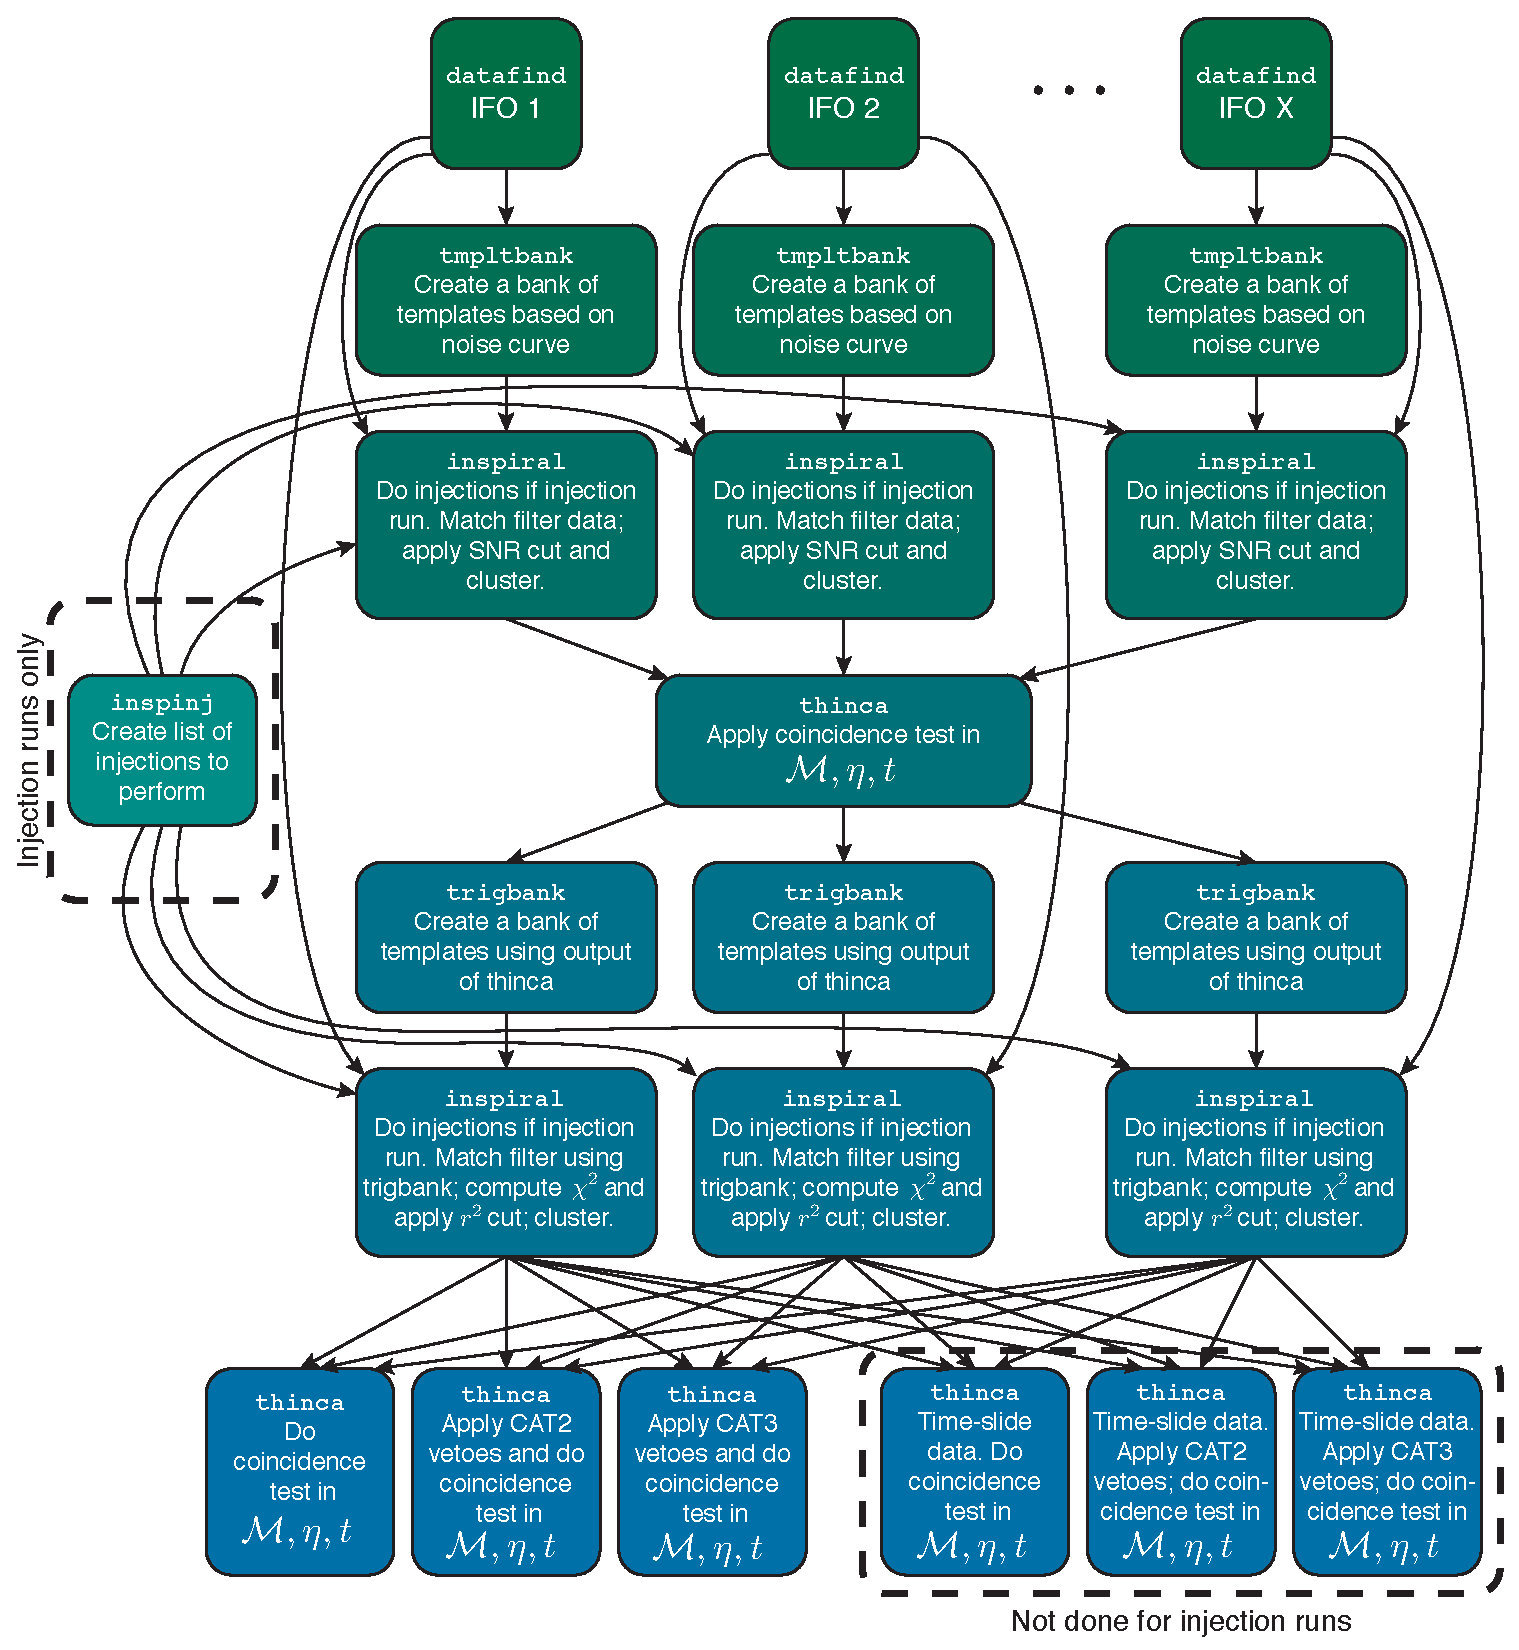
\includegraphics[width=6in]{figures/HIPEDiagram.pdf}
\end{center}
\caption{
The \ac{HIPE} pipeline. This is run once for full-data and once for
each injection run. For injection runs, \texttt{lalapps\_inspinj} is run to
generate a list of injections to create, and time slides are not done.
}
\label{fig:HIPEDiagram}
\end{figure}

\subsection{Pipedown}

After all the instances of \texttt{lalapps\_inspiral\_hipe} have run, \ihope
run \texttt{lalapps\_cbc\_pipedown} which sets up the Pipedown \ac{DAG}.
Pipedown takes the results of all the different HIPE runs, combines them into
SQLite databases, computes and ranks triggers by \ac{FAR}, and creates plots
and tables of the results. Figure \ref{fig:PipedownDiagram} details the steps
Pipedown takes to carry out these goals. Shown are the steps taken for a single
veto-category; this diagram is repated for each veto-category (by Pipedown, not
by \ihope). In-depth details of Pipedown are discussed in Section
\ref{sec:PipedownDetail}.

\begin{figure}[p]
\begin{center}
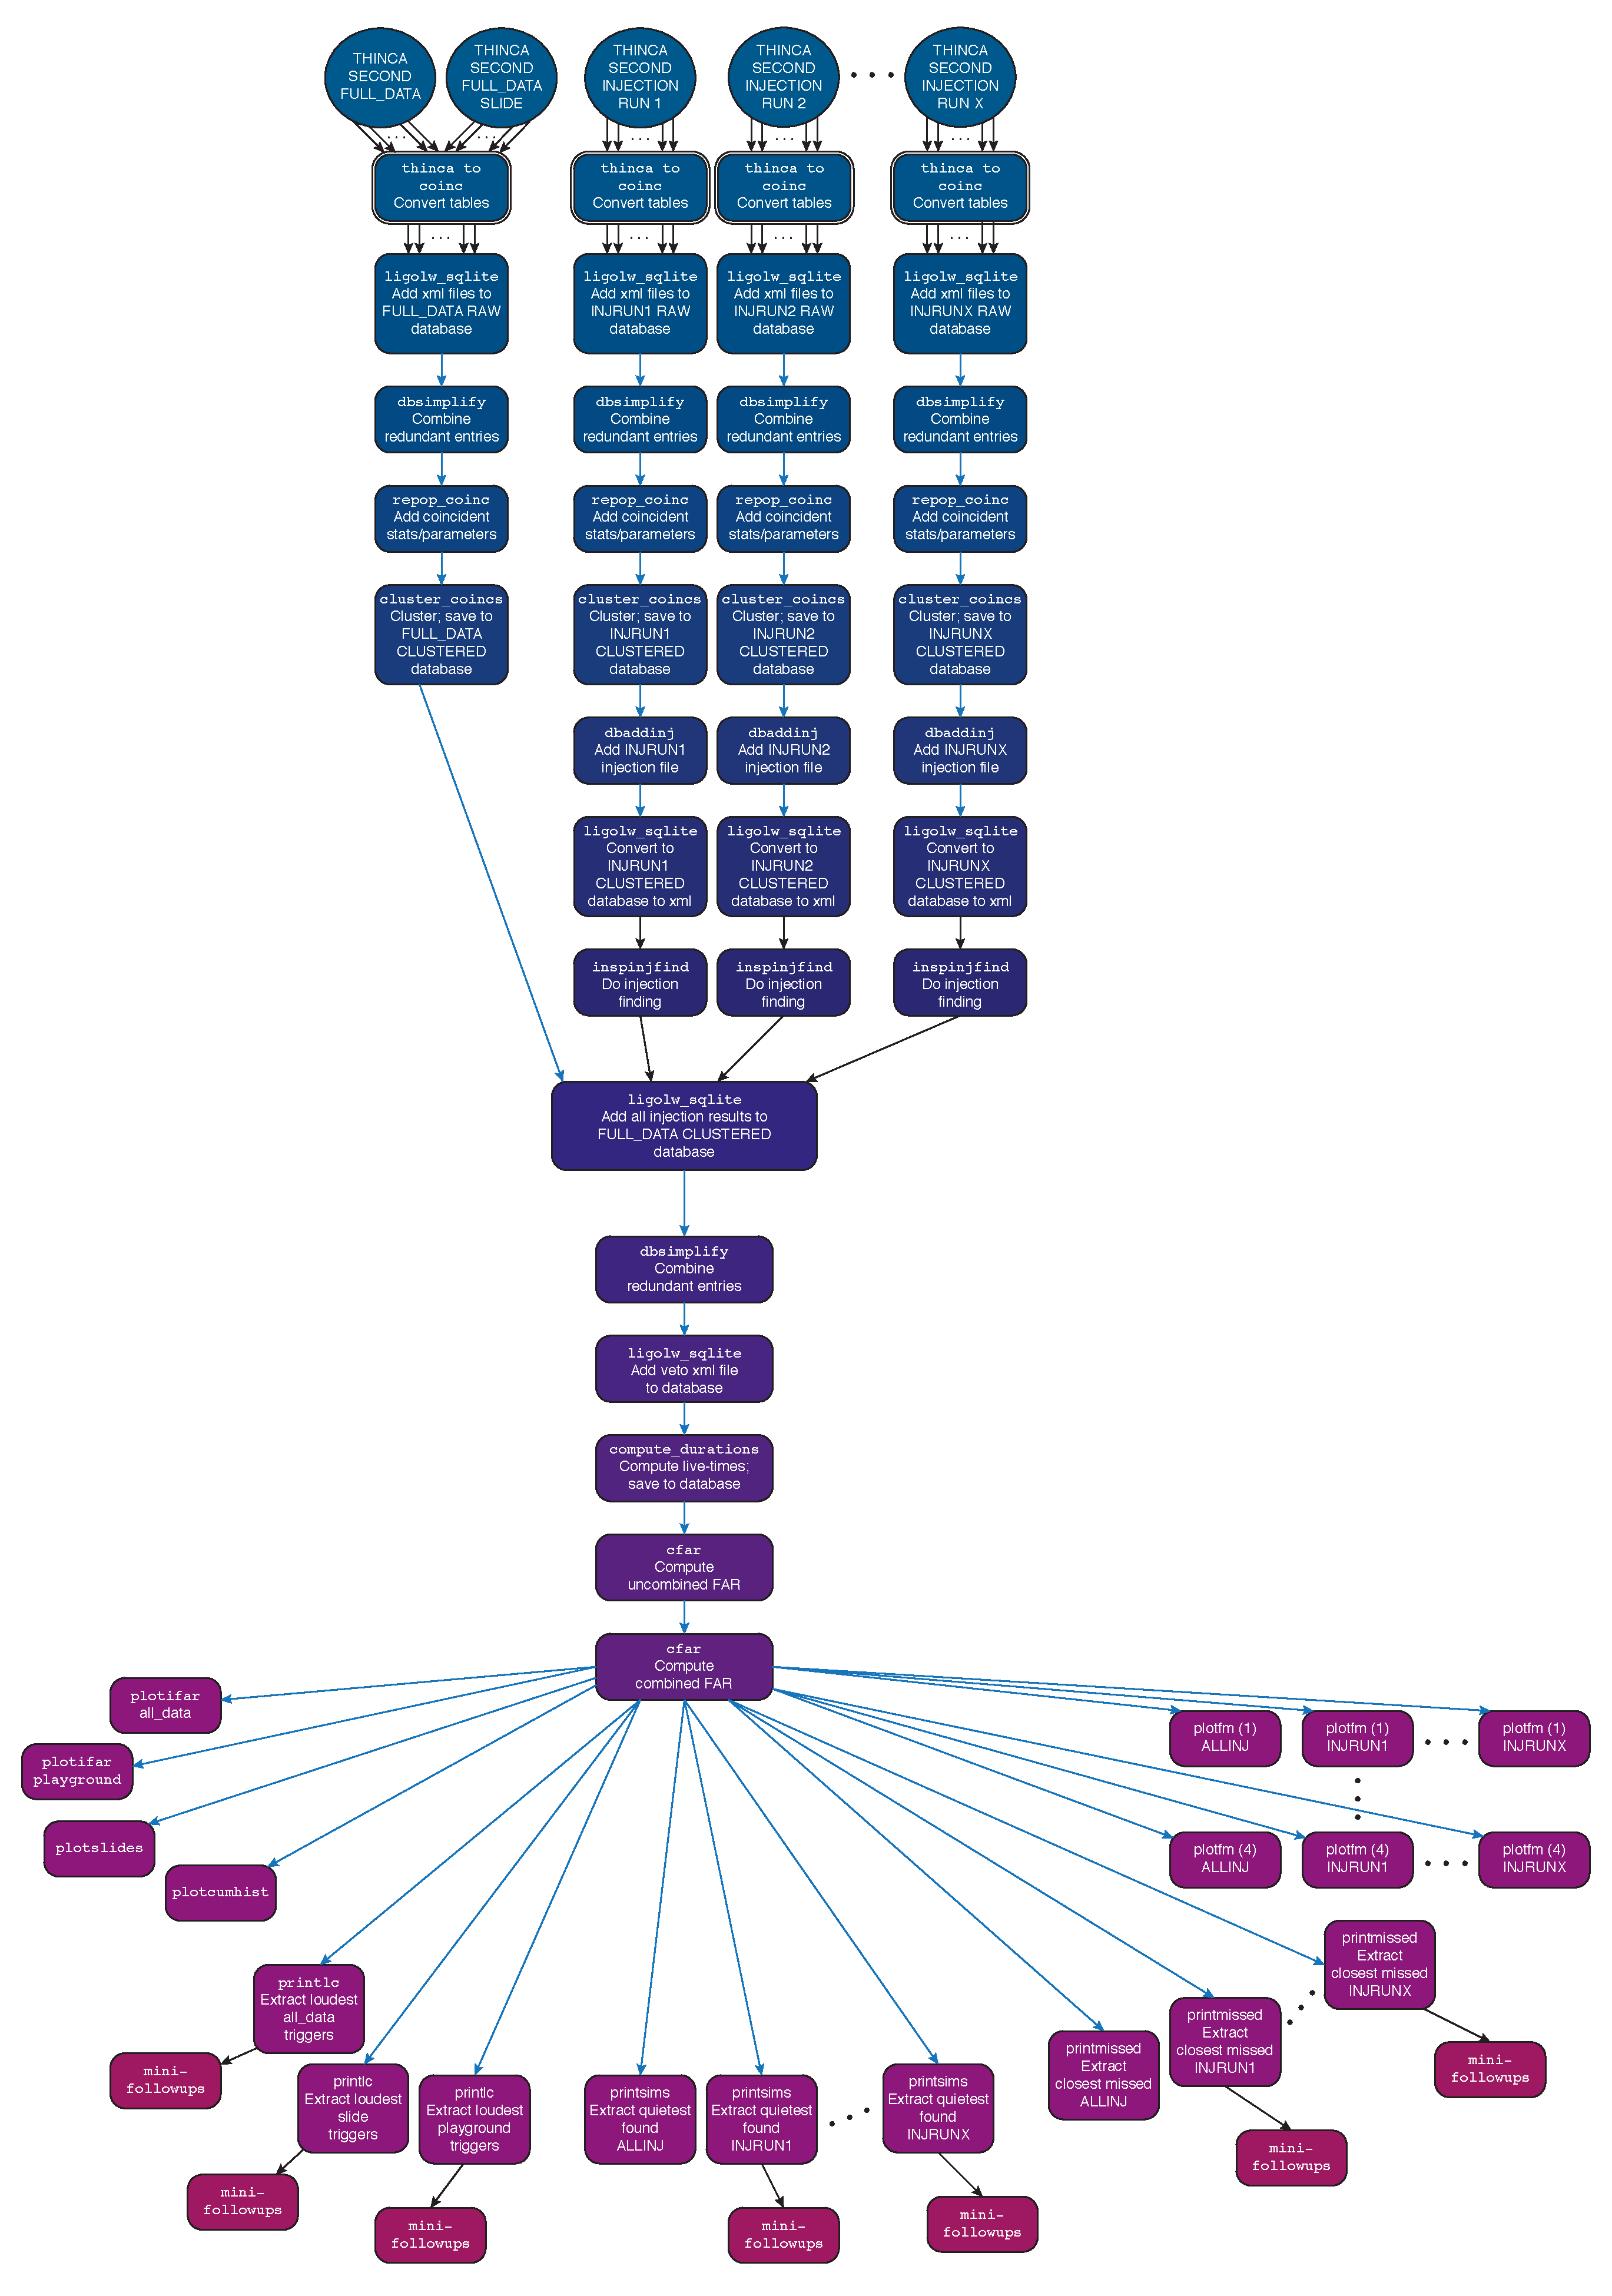
\includegraphics[width=5in]{figures/PipedownDiagram.pdf}
\end{center}
\caption{
The Pipedown pipeline for a single veto category. Each block represents a single node. Double bordered blocks represent multiple nodes. Circles represent batches of files. Black arrows represent xml files; blue arrows, SQLite databases. Each arrow represents a single file.
}
\label{fig:PipedownDiagram}
\end{figure}

\subsection{DAX}

After pipedown has completed, \ihope writes a DAX that can be used to launch the pipeline. A DAX is an abstract workflow in which elements such as file locations are variables. The DAX is turned into a \ac{DAG} by the Pegasus Workflow Management Service.

\section{HIPE in Detail}
\label{sec:HIPEdetail}

We now step through \ihope in detail, using a toy analysis of $10,240$s as an example. In this analysis we will use three interferometers: the 4-kilometer Hanford detector (H1), the 4-kilometer Livingston detector (L1), and the 3-kilometer Virgo detector (V1), and we will add one injection run, which we label \texttt{BNSINJ}. Figure \ref{fig:science-selected_segs} shows the segments that are available to analyze during this time. The \emph{selected segments} are Science segments minus CAT1 veto segments; they are what \ihope passes to \ac{HIPE} to analyze.

\begin{figure}[p]
\begin{center}
\includegraphics[width=5in]{figures/segment_plot_science-selected.pdf}
\end{center}
\caption{
The Science, category 1 vetoes, and selected segments of H1, L1, and V1 between GPS times 967228343 and 967238583.
}
\label{fig:science-selected_segs}
\end{figure}


\subsection{Data Find}

As can be seen in Figure \ref{fig:HIPEDiagram}, the first step in \ac{HIPE} is to run \texttt{lalapps\_data\_find}. Data from all of the interferometers are stored in \emph{frame files} in central locations at every computer cluster. Frame files can contain multiple channels recorded from the interferometers. For analysis purposes, we are only interested in files containing the strain data channel, which is called \texttt{LDAS-STRAIN} in the \ac{LIGO} detectors and \texttt{h\_16384Hz} in Virgo. \texttt{lalapps\_data\_find} finds the files covering the selected segments on the cluster and creates cache files listing the location of each these files in the \texttt{datafind} directory. These cache files are passed to \texttt{lalapps\_tmpltbank} and \texttt{lalapps\_inspiral}, which use them to locate and open the frame files for analysis.

\subsection{PSD Estimation and Data Segmentation}

\texttt{lalapps\_inspiral} is the program that constructs the \ac{SNR} time series for templates laid out in a bank by the program \texttt{lalapps\_tmpltbank}. The \ac{SNR} time series is constructed according to equation \ref{eqn:snr_full_form} and the templates are laid out using the metric defined in equation \ref{eqn:templateMetric}. Since both of these equations involve the inner product defined in equation \ref{eqn:inner_product}, both programs must compute the \ac{PSD}, $S_n(|f|)$, as well as the Fourier Transform of the data, $\widetilde{s}(f)$. (We do not Fourier Transform the templates. Instead, we generate the templates in the frequency domain directly by using the \ac{SPA}.)

So far, all equations we have used involving Fourier Transforms and the inner product have assumed continuous time- and frequency-domain data series. Likewise, the integrals over frequency space have been from $-\infty$ to $+\infty$. In practice, of course, the data is discreetly sampled and is neither continuous nor infinite. Both the \ac{LIGO} and Virgo strain data are sampled at $16,384\,\mathrm{Hz}$. Since even the lowest mass templates (i.e., waveforms with the highest frequency components) used in current \ac{CBC} searches terminate at frequencies around a couple of kHz, this sampling rate is much finer than is needed for our purposes. To ease computational requirements the time series is therefore downsampled to $4096\,\mathrm{Hz}$ in both \texttt{lalapps\_inspiral} and \texttt{lalapps\_tmpltbank} prior to analysis. This sampling rate sets the Nyquist frequency, $f_{\mathrm{Nyquist}}$, at $2048\,\mathrm{Hz}$. To prevent aliasing, a low-pass time-domain digital filter with a cutoff at $f_{\mathrm{Nyquist}}$ is implemented to pre-condition the data. On the low-frequency end, seismic noise dominates the interferometers' power spectrum. We therefore also impose a high-pass digital filter in the time domain. The cutoff frequency of the high-pass filter, $f_c$, is set to be a several Hz lower than a low-frequency cutoff, $f_0$, that is determined by the characteristics of each \ac{IFO}'s power spectrum. These values are set in the configuration file. (For the values chosen for \ac{S5} and \ac{S6} see Chapters \ref{ch:s5_results} and \ref{ch:s6_results}, respectively.) Both the low and high-pass filters will ring at the start and end of a time series, corrupting the data. Thus we must remove the first and last $t_{\mathrm{pad}}$ of data after applying the filters and prior to analyzing. The duration of $t_{\mathrm{pad}}$ is also set in the configuration file; for both \ac{S5} and \ac{S6} we used $8\,$s.

To Fourier Transform the data, we use the \ac{FFT} algorithm. The \ac{FFT} imposes two constraints on the data. First, the number of points in the data series must be a power of two. Second, the \ac{FFT} associates the last point of the data series with the first point; i.e., it wraps the data around on a loop. This means that as a template is slid toward the end of the time series, any points extending beyond the end of the series will be placed at the beginning. Additionally, because the last and first point of the time series are discontinuous, the wrap around essentially introduces a delta function at the end of the series. As the template passes past the discontinuity it will ring (i.e., the match filter will return the template's impulse response), and, due to the wrap around, this ringing will be placed at the beginning of the time series. Thus the first $t_{\mathrm{chirp}}$ points of the \ac{SNR} time series are corrupted, where $t_{\mathrm{chirp}}$ is the \emph{chirp length} of the template, and must be thrown out.

The chirp length is defined as the length of time it takes for the binary to go from $f_0$ to the frequency at which the binary passes \ac{ISCO}, $f_{\mathrm{isco}}$. \ac{ISCO} is the point when the separation distance is too small for the binary's masses to maintain stable orbits without external energy being added to the system; at this point the masses cease to inspiral and plunge into each other.\footnote{Note that \ac{ISCO} is not the same as the Schwarzschild radius; e.g., in a Schwarzschild space-time, \ac{ISCO} occurs at $r = 6GM/c^2$ whereas the Schwarzschild radius occurs as $r = 2GM/c^2$.} Since the \ac{pN} approximation breaks down at $f_{\mathrm{isco}}$, we must terminate all integrals at this point. Combining this with the realities of Nyquist and seismic noise, all frequency domain integrals are limited to the region $f \in [f_0, f_{\mathrm{max}})$ where $f_{\mathrm{max}} = \min(f_{\mathrm{Nyquist}},~f_{\mathrm{isco}})$.

The \ac{PSD} is estimated using Welch's method. This involves breaking a data segment up into several bins of equal duration. Within each bin, the data is transformed to the frequency domain via the \ac{FFT}. Thus the number of points in each bin must be a power of two, and the bins must be overlapping to account for the wrap-around corruption at the beginning and end of each segment. Since the data is discreet, this results in a discreet number of frequency bins. The \emph{median} value within each frequency bin is then chosen across all the data segments to construct $S_n(|f|)$. We use the medain --- as opposed to the mean --- to better buffer the \ac{PSD} from over-estimation in the prescence of a signal.

As was the case with the template, $S_n(|f|)$ will be corrupted by the discontinuity between the first and last point of the data series. However, unlike the template, which has a finite duration, $S_n(|f|)$ will ring for the entire data segment. This ringing will also happen if a delta-function like glitch exists in the data. To prevent the entire segment from being corrupted, we \emph{truncate} the \ac{PSD}. This is done by estimating \ac{PSD} using Welch's method, inverse transforming $\sqrt{S_n^{-1}(|f|)}$ to the time domain, zeroing out the first and last $t_{\mathrm{invspectrunc}}$ seconds of the time series, then transforming back to the frequency domain. This limits the corruption due to the wraparound to the first and last $t_{\mathrm{invspectrunc}}$ seconds of the time series. The truncation does cause some smoothing out of high Q features, such as power-line harmonics; however, since we search for relatively broad band signals this smoothing has little effect on the search. The value of $t_{\mathrm{invspectrunc}}$ was set to $8\,$s for both \ac{S5} and \ac{S6}.

For more details on \ac{PSD} estimation and implementation of the matched filter with a discreet and finite time-series, see \cite{ref:Brown} and \cite{ref:FindChirp}.

\subsection{Template Bank and Inspiral}

We therefore identify \emph{triggers} by selecting points when $\rho(t)$ is maximum. This is done by using the \emph{max over chirp length} algorithm. Max over chirp length uses a sliding time window to select triggers: for every point in time, a point is only kept if there is no other point with a $\rho$ greater than it within the \emph{chirp length} of the template. $f_0$ is selected based on when the detector's \ac{PSD} effectively goes to infinity due to low-frequency seismic noise. In intial LIGO, $f_0$ is set to $40\,\mathrm{Hz}$; for advanced LIGO it is expected to be $10\,\mathrm{Hz}$. Once a trigger is identified, the time at which it occurs is associated with the \emph{coalescence}, or \emph{end-time}, $t_c$, of the binary.

For \ac{S5} and \ac{S6}, we laid out templates on a hexagonal grid using non-spinning 2\ac{pN} waveforms to calculate the metric \cite{?}. The gridding was chosen so that the overlap between two neighboring templates was $94\%$, giving a maximum \ac{SNR} loss of $3\%$. This resulted in a maximum loss in sensitive volume due to the discreetness of the bank of $\sim10\%$.

